\section{Beyond Just an Integral: A New Definition of Measurability}

But this raised an even deeper question:

\begin{quote}
\textbf{If Riemann integration failed for certain functions, then what exactly makes a function measurable in the Lebesgue sense?}
\end{quote}

 to fully define Lebesgue integration, mathematicians had to formalize the very concept of measurable sets—establishing a rigorous way to determine when a function could be integrated at all.

This leads us directly to the core idea behind Lebesgue’s method: \textbf{measurable sets and inclusion maps}.

\subsection{The Key Idea: Measurable Sets and Inclusion Maps}

In order for a function to be \textbf{Lebesgue integrable}, the set of points where the function takes certain values must be \textbf{measurable}. This means that there must exist a measure-preserving \textbf{inclusion map} into a well-behaved space (such as the real numbers with standard Lebesgue measure).

Formally, a function \( f: \mathbb{R} \to \mathbb{R} \) is measurable if for every real number \( a \), the preimage set

\[
\{ x \mid f(x) > a \}
\]

is a \textbf{Lebesgue measurable set}—meaning it can be covered by open intervals whose total measure matches its "size" as closely as possible.

\begin{figure}[h]
    \centering
    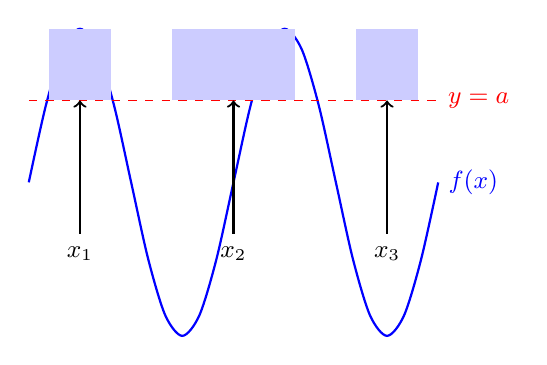
\begin{tikzpicture}[scale=1.3]

        % Function curve
        \draw[thick, domain=-2:2, smooth, variable=\x, blue] plot ({\x}, {1.5*sin(180*\x)}) node[right] {\small $f(x)$};

        % Horizontal line at y=a
        \draw[dashed, red] (-2,0.8) -- (2,0.8);
        \node[red, right] at (2,0.8) {\small $y = a$};

        % Preimage set: { x | f(x) > a }
        \fill[blue!20] (-1.8,0.8) -- (-1.2,0.8) -- (-1.2,1.5) -- (-1.8,1.5) -- cycle;
        \fill[blue!20] (-0.6,0.8) -- (0.6,0.8) -- (0.6,1.5) -- (-0.6,1.5) -- cycle;
        \fill[blue!20] (1.2,0.8) -- (1.8,0.8) -- (1.8,1.5) -- (1.2,1.5) -- cycle;

        % Arrows to indicate inclusion into the real line
        \draw[->, thick] (-1.5,-0.5) -- (-1.5,0.8);
        \draw[->, thick] (0,-0.5) -- (0,0.8);
        \draw[->, thick] (1.5,-0.5) -- (1.5,0.8);

        % Labels
        \node at (-1.5,-0.7) {\small $x_1$};
        \node at (0,-0.7) {\small $x_2$};
        \node at (1.5,-0.7) {\small $x_3$};

    \end{tikzpicture}
\caption{The function \( f(x) \) (blue) is Lebesgue measurable if the preimage set \( \{ x \mid f(x) > a \} \) (blue-shaded regions) can be covered by measurable intervals. The red dashed line represents a threshold \( y = a \), and the arrows indicate inclusion into the real line.}
\end{figure}


If such an \textbf{inclusion map} into a measurable space exists, then the function is Lebesgue integrable. If not, the function is so irregular that it defies any reasonable notion of size or integration—just like Dirichlet’s function, where the inclusion maps fail to exist in a well-defined way.

\subsection{An Intuitive Analogy: Sorting Puzzle Pieces into Fitting Boxes}

Imagine you have a massive pile of puzzle pieces of all different shapes and sizes. Some pieces are regular, like squares and rectangles, while others are jagged and irregular. Your goal is to store them neatly in containers.

\begin{itemize}
    \item If a piece has a predictable shape, like a square, it easily fits into a standard box.
    \item If a piece is slightly irregular, you might need a flexible container, but it still fits.
    \item However, if the piece is extremely jagged—so much so that it doesn’t fit into any reasonable box—it becomes impossible to store properly.
\end{itemize}

\textbf{This is like the idea of measurable sets and inclusion maps.} 

- The "box" represents a well-behaved space where we can measure things properly (such as the real numbers with standard Lebesgue measure).
- The puzzle pieces represent different sets of points where the function takes certain values.
- If a function’s values can be mapped into a well-behaved measurable space (i.e., the pieces fit into some structured container), then it is measurable and integrable.
- But if the function is too irregular—like an infinitely jagged puzzle piece that won’t fit in any box—then it cannot be measured in the Lebesgue sense.

 just as some puzzle pieces can be neatly sorted while others resist organization, some functions can be properly measured, while others (like Dirichlet’s function) are too chaotic to fit into the standard framework.
 
 \begin{center}
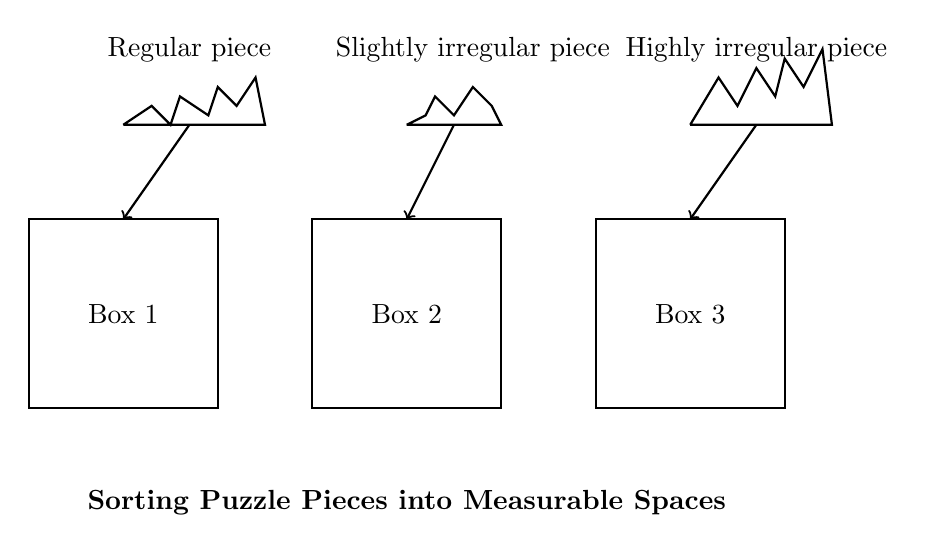
\begin{tikzpicture}[scale=1.2]

    % Draw containers (well-behaved spaces)
    \draw[thick] (0,0) rectangle (2,2) node[pos=.5] {Box 1};
    \draw[thick] (3,0) rectangle (5,2) node[pos=.5] {Box 2};
    \draw[thick] (6,0) rectangle (8,2) node[pos=.5] {Box 3};
    
    % Draw puzzle pieces
    \draw[thick] (1,3) -- (1.3,3.2) -- (1.5,3) -- (1.6,3.3) -- (1.9,3.1) -- (2,3.4) -- (2.2,3.2) -- (2.4,3.5) -- (2.5,3) -- (1,3);
    \draw[thick] (4,3) -- (4.2,3.1) -- (4.3,3.3) -- (4.5,3.1) -- (4.7,3.4) -- (4.9,3.2) -- (5,3) -- (4,3);
    \draw[thick] (7,3) -- (7.3,3.5) -- (7.5,3.2) -- (7.7,3.6) -- (7.9,3.3) -- (8,3.7) -- (8.2,3.4) -- (8.4,3.8) -- (8.5,3) -- (7,3);

    % Arrows mapping puzzle pieces into boxes
    \draw[->, thick] (1.7,3) -- (1,2);
    \draw[->, thick] (4.5,3) -- (4,2);
    \draw[->, thick] (7.7,3) -- (7,2);

    % Labels
    \node at (1.7,3.8) {Regular piece};
    \node at (4.7,3.8) {Slightly irregular piece};
    \node at (7.7,3.8) {Highly irregular piece};

    \node at (4,-1) {\textbf{Sorting Puzzle Pieces into Measurable Spaces}};
    
\end{tikzpicture}
\end{center}

\begin{quote}
\textbf{Figure: Sorting Puzzle Pieces into Measurable Spaces.}  
The boxes represent well-behaved measurable spaces, while the puzzle pieces symbolize different sets of function values. Regular and slightly irregular pieces fit neatly into structured containers, illustrating functions that can be measured using Lebesgue integration. However, the highly irregular piece resists fitting into any box, representing functions too chaotic to be properly measured. Just as some puzzle pieces are easy to organize while others defy storage, some functions can be integrated, while others, like Dirichlet’s function, remain beyond reach.
\end{quote}


\subsection{Why This Matters: A Real-World Problem That Needed Lebesgue’s Solution}

Understanding measurable sets and inclusion maps might seem abstract, but these ideas arose from real scientific challenges. One such problem was radioactive decay, a major topic in early 20th-century physics. 

In 1905, physicists needed to answer:

\begin{quote}
\textit{"If we have a sample of radium, how long should we expect a single atom to survive before it decays?"}
\end{quote}

Radioactive decay follows an \textbf{exponential distribution}, where the probability density function (PDF) for the lifetime \( X \) of a radium atom is:

\[
f(t) = \lambda e^{-\lambda t}, \quad t \geq 0
\]

where \( \lambda \) is the decay constant.

The expected lifetime of a radium atom is given by:

\[
E[X] = \int_0^\infty t f(t) \, dt = \int_0^\infty t \lambda e^{-\lambda t} \, dt
\]

\begin{figure}[h]
    \centering
    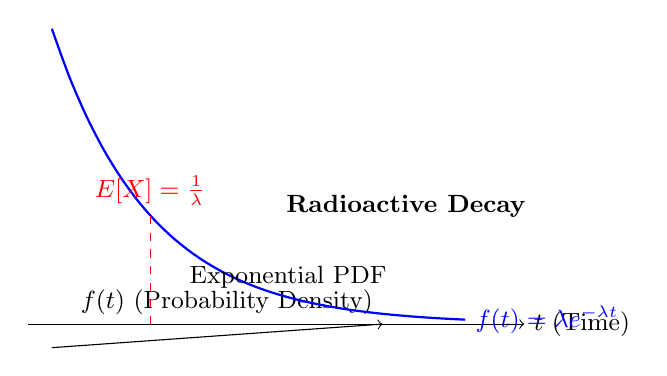
\begin{tikzpicture}[scale=1.5]

        % Axes
        \draw[->] (-0.2, 0) -- (4, 0) node[right] {\small $t$ (Time)};
        \draw[->] (0, -0.2) -- (2.8, 0) node[above left] {\small $f(t)$ (Probability Density)};

        % Exponential Decay Function
        \draw[thick, domain=0:3.5, smooth, variable=\x, blue] plot ({\x}, {2.5*exp(-1.2*\x)}) node[right] {\small $f(t) = \lambda e^{-\lambda t}$};

        % Expected Value Indicator
        \draw[dashed, red] (1/1.2, 0) -- (1/1.2, {2.5*exp(-1.2*(1/1.2))}) node[above] {\small $E[X] = \frac{1}{\lambda}$};

        % Labels
        \node at (3, 1) {\small \textbf{Radioactive Decay}};
        \node at (2, 0.4) {\small Exponential PDF};

    \end{tikzpicture}

    \caption{The probability density function \( f(t) = \lambda e^{-\lambda t} \) models the exponential decay of a radium atom's lifetime. The expected value, marked in red, is \( E[X] = \frac{1}{\lambda} \), representing the average lifetime of an atom before decay.}
\end{figure}


\subsection{Why Riemann Integration Fails}

Riemann integration, which sums rectangles along the x-axis, struggles with this because:

\begin{itemize}
    \item The probability mass is not uniformly distributed, making x-axis partitions inefficient.
    \item The integral spans an infinite range, making it difficult to approximate with finite sums.
    \item Classical probability methods based on discrete counting fail for continuous decay times.
\end{itemize}

\subsection{How Lebesgue Integration Solves the Problem}

Lebesgue’s insight was to sum over function values instead of partitioning the x-axis. Using measure-theoretic probability, expectation is redefined as:

\[
E[X] = \int_{\Omega} X(\omega) \, dP(\omega)
\]

Since \( dP(x) = f(x) \, dx \), the expectation simplifies to:

\[
E[X] = \int_0^\infty t \lambda e^{-\lambda t} \, dt
\]

Using integration by parts:

\[
E[X] = \frac{1}{\lambda}
\]

\begin{figure}[h]
    \centering
    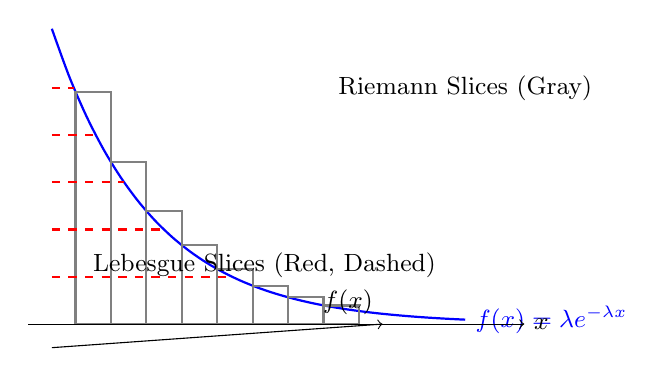
\begin{tikzpicture}[scale=1.5]

        % Define function
        \draw[thick, domain=0:3.5, smooth, variable=\x, blue] plot ({\x}, {2.5*exp(-1.2*\x)}) node[right] {\small $f(x) = \lambda e^{-\lambda x}$};

        % Riemann Slices (Vertical Strips)
        \foreach \x in {0.2, 0.5, 0.8, 1.1, 1.4, 1.7, 2.0, 2.3} {
            \draw[gray, thick] (\x, 0) -- (\x, {2.5*exp(-1.2*\x)}) -- ({\x+0.3}, {2.5*exp(-1.2*\x)}) -- ({\x+0.3}, 0) -- cycle;
        }

        % Lebesgue Slices (Horizontal Strips)
        \foreach \y in {0.4, 0.8, 1.2, 1.6, 2.0} {
            \draw[red, thick, dashed] (0, \y) -- ({ln(2.5/\y)/1.2}, \y);
        }

        % Axes
        \draw[->] (-0.2, 0) -- (4, 0) node[right] {\small $x$};
        \draw[->] (0, -0.2) -- (2.8, 0) node[above left] {\small $f(x)$};

        % Labels
        \node at (3.5, 2) {\small Riemann Slices (Gray)};
        \node at (1.8, 0.5) {\small Lebesgue Slices (Red, Dashed)};

    \end{tikzpicture}

    \caption{The diagram compares Riemann integration (gray vertical slices) with Lebesgue integration (red horizontal slices) using the exponential probability density function \( f(x) = \lambda e^{-\lambda x} \). Riemann integration partitions the **x-axis** into small intervals and sums the areas, while Lebesgue integration groups all \( x \)-values where the function takes a particular value, making it more flexible for probability measures. This approach naturally aligns with expectation calculations in measure-theoretic probability.}
\end{figure}

